\section{薄透镜与光组的基本描述}

\subsection{从两个折射面到一个薄透镜}

本讲先研究近轴成像，再讨论能精确成像的特殊曲面。近轴计算同时要求光线与主轴夹角小、折射点高度相对曲率半径小；“薄”还要求透镜厚度对所研究的物像关系可以忽略。这两个近似须分别判断。

沿本次传播方向取正，实物距 \(u>0\)，虚物距 \(u<0\)；实像距 \(v>0\)，虚像距 \(v<0\)。物高和像高 \(h,h'\) 均带符号，横向放大率定义为 \(\beta=h'/h\)。左右介质相同的薄透镜满足
\begin{equation}\label{eq:o3thin}
 \boxed{\frac1u+\frac1v=\frac1f},\qquad
 \boxed{\beta=-\frac vu}.
\end{equation}
会聚透镜 \(f>0\)，发散透镜 \(f<0\)。实物在会聚透镜焦点上时，出射为平行光，不能给它指定有限像高和有限像距。

\fig{o3:two-surfaces}{先按同一传播方向判断两个球心；厚度在结构图中放大，薄镜计算才把两量距平面合并}{\begin{tikzpicture}

\draw[axis](-3,0)--(3,0)node[right]{$+x$};\fill[blue!10]plot[domain=-.85:.85,samples=60]({1.8-sqrt(4-(\x)^2)},\x)--plot[domain=.85:-.85,samples=60]({-1.8+sqrt(4-(\x)^2)},\x)--cycle;
\draw[world,domain=-.85:.85,samples=60]plot({1.8-sqrt(4-(\x)^2)},\x);\draw[world,domain=-.85:.85,samples=60]plot({-1.8+sqrt(4-(\x)^2)},\x);\draw[normal](-.13649,.5)--(1.8,0);\draw[normal](.13649,.5)--(-1.8,0);\fill(1.8,0)circle(1.5pt)node[below]{$C_1$};\fill(-1.8,0)circle(1.5pt)node[below]{$C_2$};\node[above left]at(-.13649,.5){$P_1$};\node[above right]at(.13649,.5){$P_2$};\node at(-2,1.4){$R_1>0$};\node at(2,1.4){$R_2<0$};\node at(-2,-.7){$n_0$};\node at(2,-.7){$n_0$};\node at(0,-.5){$n$};\draw[dim](-.2,-1.1)--(.2,-1.1)node[midway,below]{$t\to0$};

\end{tikzpicture}}
图\ref{o3:two-surfaces}的第一面球心在出射侧，第二面球心在入射侧，故双凸结构的两半径号相反。计算中先保留各面的介质顺序与中间像，最后才令 $t\to0$；“双凸”这一个形状名称不能代替两个曲率号。


薄透镜公式可以由两个球面折射式相加得到。设透镜折射率为 $n$、两侧均为 $n_0$，两面的带符号半径为 $R_1,R_2$。忽略厚度时，第一面中间像距为 $v_1$，第二面的物距就是 $u_2=-v_1$。于是
\[
 \frac{n_0}{u}+\frac n{v_1}=\frac{n-n_0}{R_1},\qquad
 -\frac n{v_1}+\frac{n_0}{v}=\frac{n_0-n}{R_2}.
\]
相加消去中间像，得到
$1/f=(n/n_0-1)(1/R_1-1/R_2)$，再得到式\eqref{eq:o3thin}。这说明焦距来自两次折射的共同作用，透镜厚度可略才允许把两个量距起点合并。

当 $n_0$ 改变，透镜的焦距和会聚性质也可能改变；不能只按几何外形决定焦距正负。若厚度已不能忽略，中间像距也不能直接反号作为第二面物距，必须保留两面间隔，或改用光组的主平面描述。

\subsection{三条辅助光线及其条件}

在两侧同一介质中的薄透镜，穿过光心 \(O\) 的近轴光线方向不变；平行主轴的入射光经会聚透镜后通过像方焦点 \(F'\)；经物方焦点 \(F\) 入射的光出射后平行主轴。发散透镜的焦点须用相应延长线理解。左右介质不同时，过光心的光线一般会改变倾角，不能继续使用“直穿光心”的规则。
\fig{fig:o3special}{两侧均为空气的会聚薄透镜；三条光线在同一像点相交}{
\begin{tikzpicture}[x=1.25cm,y=1cm]
\draw[axisline] (-3.5,0)--(2.2,0);
\draw[<->,>=Stealth,world] (0,-1)--(0,1.1);
\draw[axis,thick] (-3,0)--(-3,.6) node[above] {$A$};
\draw[axis,thick] (1.5,0)--(1.5,-.3) node[below] {$A'$};
\draw[ray] (-3,.6)--(0,.6);\draw[ray] (0,.6)--(1.5,-.3);
\draw[ray] (-3,.6)--(0,0);\draw[ray] (0,0)--(1.5,-.3);
\draw[ray] (-3,.6)--(0,-.3);\draw[ray] (0,-.3)--(1.5,-.3);
\node[below] at (-1,0) {$F$};\node[above right] at (0,0) {$O$};
\node[above] at (1,0) {$F'$};
\end{tikzpicture}}
图\ref{fig:o3special}中，\(A'\) 是实际光线的交点，故为实像；它在轴下，故 \(\beta<0\)。只有反向延长线相交时才是虚像，虚线不能代替实际传播方向。

这三条线都来自同一个近轴光线变换。穿过光心的一条不偏折，并不是所有过透镜中心附近的光线都不折射，而是薄透镜、两侧介质相同条件下，两次小偏折在方向上抵消。若有明显厚度，出射线可能与入射线平行但横向错开；把这段错位忽略后才画成一条直线。

作虚像时，先从物点画到透镜，再沿出射方向画真实半直线，最后向后延长求交点。延长线的交点只决定观察者追溯的位置，不能把它改画成光在透镜前实际交叉。辅助光线也必须穿过有效孔径；若被镜框挡住，应换一条允许光线求像，几何成像位置与通光范围分别检查。

\subsection{实像、虚像与会聚性质的区别}

“会聚透镜”表示它使近轴光束的会聚度增加，并不保证任何入射束都在右侧形成实像。以实物为例，会聚镜 $v=fu/(u-f)$ 在 $u=f$ 处经过平行出射状态：$u>f$ 时成实像，$0<u<f$ 时成正立放大虚像。发散镜对实物成正立缩小虚像。图\ref{o3:virtual-images}先画实际出射半直线，再反向延长，像的虚实与正倒由两个不同的几何关系决定。
\fig{o3:virtual-images}{实物的两种虚像：左为会聚镜焦内成像，右为发散镜成像；虚线只用于求交点}{\begin{tikzpicture}

\begin{scope}[scale=.85]
\draw[axisline](-2.7,0)--(2,0);\draw[<->,>=Stealth,world](0,-.9)--(0,1.25);\draw[axis,blue](-.6,0)--(-.6,.3)node[above]{$B$};\draw[axis,red,dashed](-1.5,0)--(-1.5,.75)node[above]{$B'$};\draw[ray](-.6,.3)--(0,0);\draw[ray](0,0)--(1.7,-.85);\draw[virtual](-1.5,.75)--(0,0);\draw[ray](-.6,.3)--(0,.3);\draw[ray](0,.3)--(1.7,-.21);\draw[virtual](-1.5,.75)--(0,.3);\node[below]at(-1,0){$F$};\node[below right]at(0,0){$O$};\node at(-.5,-1.5){$0<u<f,\quad\beta>1$};\end{scope}
\begin{scope}[xshift=5.5cm,scale=.85]
\draw[axisline](-3.5,0)--(2,0);\draw[world](0,-.9)--(0,1.25);\draw[axis,blue](-3,0)--(-3,.6)node[above]{$B$};\draw[axis,red,dashed](-.75,0)--(-.75,.15);\draw[ray](-3,.6)--(0,0);\draw[ray](0,0)--(1.7,-.34);\draw[virtual](-.75,.15)--(0,0);\draw[ray](-3,.6)--(0,.6);\draw[ray](0,.6)--(1.7,1.62);\draw[virtual](-1,0)--(0,.6);\node[below]at(-1,0){$F'$};\node[below right]at(0,0){$O$};\draw[aux](-.75,.15)--(-1.5,.8);\node[above]at(-1.5,.8){$B'$};\node at(-.5,-1.5){$f<0,\quad0<\beta<1$};\end{scope}

\end{tikzpicture}}
两侧介质相同时，过光心的光线保持方向，可以连接物高与像高。透镜正负则应由平行入射束的出射会聚度判断。后文组合系统还会出现负透镜接收虚物而成实像的情形，应继续按入射、出射两束光分别判断。


\subsection{主平面与物像距的测量}

有厚度的透镜或多个透镜组成的光组，在近轴范围可用主平面 \(H,H'\) 与焦点 \(F,F'\) 描述。物距从 \(H\) 量，像距从 \(H'\) 量；两者均不必从最外侧镜面顶点量。图中把对应光线从 \(H\) 平移到 \(H'\) 是等效作图，不能据此断言光在仪器内部沿水平线传播。

设左右介质折射率为 \(n_u,n_v\)，光焦度为 \(\Phi\)，则
\[
 \boxed{\frac{n_u}{u}+\frac{n_v}{v}=\Phi},\qquad
 f_u=\frac{n_u}{\Phi},\quad f_v=\frac{n_v}{\Phi},
 \qquad \frac{f_u}{u}+\frac{f_v}{v}=1.
\]
这里 \(f_u,f_v\) 为按会聚性质赋号的焦距。会聚光组中，\(F\) 在 \(H\) 左侧，\(F'\) 在 \(H'\) 右侧，而两段焦距都取正。\(\Phi=0\) 的无焦系统须直接分析光束传递，不再代入有限焦距形式。

\fig{fig:o3principal-distance}{主平面是等效量距基准，与外表面顶点分别标出}{\begin{tikzpicture}
\fill[gray!8](0,-.9)rectangle(3,.9);\draw[world](0,-.9)rectangle(3,.9);
\draw[axisline](-2.7,0)--(6.2,0);
\draw[normal](.8,-1.3)--(.8,1.3)node[above]{$H$};
\draw[normal](2.1,-1.3)--(2.1,1.3)node[above]{$H'$};
\fill(-2,0)circle(1.5pt)node[above]{$S$};\fill(5.6,0)circle(1.5pt)node[above]{$S'$};
\node[below left]at(0,0){$O_1$};\node[below right]at(3,0){$O_2$};
\draw[dim](-2,-1.65)--(.8,-1.65)node[midway,below]{$u$};
\draw[dim](2.1,-1.65)--(5.6,-1.65)node[midway,below]{$v$};
\node at(1.45,.5){光组};
\end{tikzpicture}}
图\ref{fig:o3principal-distance}将外表面顶点与两主平面分开。测得物体到前表面的距离后，还须加上或减去该表面到 $H$ 的有向偏移，才能代入等效成像式。像侧也同样处理。主平面是整个光组的等效性质，未必落在镜片材料内；不能通过把图中的虚线画得更像一片透镜来决定它的位置。

物方焦点与像方焦点分别由一侧出射平行和一侧入射平行定义。外界介质不同时，两焦距之比为 $n_u/n_v$，它们对应同一个光焦度。若把两焦距都强行取成同一个数，就会破坏介质次序和放大率中的折射率因子。

\subsection{用高度和约化倾角逐级计算}

令光线高度为 \(y\)，小倾角为 \(\theta\)，约化倾角为 \(p=n\theta\)。在均匀介质内传播距离 \(d\)，以及通过近轴折射面时，分别有
\[
 \binom{y_2}{p_2}=\begin{pmatrix}1&d/n\\0&1\end{pmatrix}\binom{y_1}{p_1},
 \qquad
 \binom{y_+}{p_+}=\begin{pmatrix}1&0\\-\Phi_s&1\end{pmatrix}\binom{y_-}{p_-},
\]
其中 \(\Phi_s=(n_+-n_-)/R_s\)，球心在本次出射侧时 \(R_s>0\)。薄透镜可把两个面的光焦度相加。多个元件依次作用时，应先按传播顺序组成总矩阵，再在指定物、像平面之间判断成像。
初学时先沿实际传播方向逐级标出物、像及量距起点，再列各面的成像式。熟悉这条主线后，可用矩阵复算，或把矩阵用于分离光组的主平面与焦距；计算简写不能替代实物、虚物的判断。

镜面反射后传播方向改变，应重新定义下一段的物距和曲率符号。镀银透镜要经历两次透镜折射，不能只把它当作一次透镜再接一个普通反射镜。

矩阵乘法的顺序应与实际传播次序对应。若光线先经过面1、再传播距离 $d$、最后经过面2，总矩阵为 $M_2P(d)M_1$，最先作用的矩阵写在最右边。传播使高度变化而约化倾角不变，界面折射使倾角变化而交点高度连续；这正是两类基本矩阵中零元和单位元的物理意义。

总关系为 $y_{\rm out}=Ay_{\rm in}+Bp_{\rm in}$。同一物点可以发出不同倾角的光，成像要求它们到达同一像高，因此必须消去对 $p_{\rm in}$ 的依赖，即 $B=0$，此时横向放大率就是 $A$。这些基本矩阵的行列式均为一，总矩阵也应满足 $AD-BC=1$，可以独立检查乘法次序或系数错误。矩阵给出数值关系后，仍要回到实际光路判定是否被孔径遮挡。

\fig{fv:o3:matrix}{传播改变高度，薄透镜在同一高度改变光线倾角}{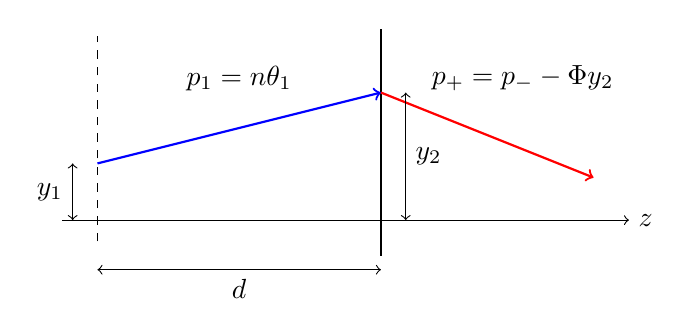
\begin{tikzpicture}[scale=.9]
\draw[->](-.5,0)--(7.5,0)node[right]{$z$};\draw[dashed](0,-.3)--(0,2.6);\draw[thick](4,-.5)--(4,2.7);
\draw[->,blue,thick](0,.8)--(4,1.8);\draw[->,red,thick](4,1.8)--(7,.6);
\draw[<->](0,-.7)--(4,-.7)node[midway,below]{$d$};
\draw[<->](-.35,0)--(-.35,.8)node[midway,left]{$y_1$};\draw[<->](4.35,0)--(4.35,1.8)node[midway,right]{$y_2$};
\node at(2,2){$p_1=n\theta_1$};\node at(6,2){$p_+=p_- -\Phi y_2$};
\end{tikzpicture}}
图\ref{fv:o3:matrix}把矩阵中的每一项落实到光线：均匀段有 $y_2-y_1=d\tan\theta_1\simeq dp_1/n$，倾角不变；薄透镜处高度连续，约化倾角突变 $-\Phi y_2$。所以从左向右追迹时，先作用的传播矩阵写在右边，后作用的透镜矩阵写在左边。若把次序颠倒，透镜使用的高度会由 $y_2$误变为 $y_1$，一般对应另一套装置。这个几何顺序是矩阵乘法次序的依据。


由两种基本矩阵还可看出镜厚的影响。设两球面光焦度为 $\Phi_1,\Phi_2$，玻璃内厚度为 $t$、折射率为 $n$。总矩阵为
\[
M=\begin{pmatrix}1&0\\-\Phi_2&1\end{pmatrix}
\begin{pmatrix}1&t/n\\0&1\end{pmatrix}
\begin{pmatrix}1&0\\-\Phi_1&1\end{pmatrix},
\]
先乘右边两个矩阵，再乘最左矩阵：
\[
P(t/n)M_1=
\begin{pmatrix}1-t\Phi_1/n&t/n\\-\Phi_1&1\end{pmatrix},
\]
\[
M=
\begin{pmatrix}
1-t\Phi_1/n&t/n\\
-\Phi_2(1-t\Phi_1/n)-\Phi_1&1-t\Phi_2/n
\end{pmatrix}.
\]
左下元为 $C=-\Phi_2+t\Phi_1\Phi_2/n-\Phi_1$，故 $\Phi_{\rm eff}=-C$ 给出
\[
\Phi_{\rm eff}=\Phi_1+\Phi_2-\frac tn\Phi_1\Phi_2.
\]
零厚度时才严格回到光焦度直接相加；若两面作用接近相消，厚度修正相对净光焦度可能很大，即使结构上看起来很薄，也要检查所求精度。


\subsection{会聚入射束与第二级的虚物}

组合系统中，第一级算出的像点首先表示它单独作用时的会聚目标。第二镜若放在这个目标之前，光还没有到达目标便再次折射，因此目标对第二镜而言是虚物，而不是已经存在的发光物体。

图\ref{fig:o3-virtual-geometry}中，第一镜的单独像为 $B_1$，两镜间距为 $d$。以第一镜位置为轴向原点，则第二镜物距为
\[
 u_2=d-v_1.
\]
当 $v_1>d$ 时，$u_2<0$；这来自光束正在会聚，不表示光已从右向左传播。虚线保留撤去第二镜时的路径，实际光路必须沿实线箭头追迹。
\fig{fig:o3-virtual-geometry}{负透镜可以减弱已有的会聚度，虚物情形下仍可能得到实像}{
\begin{tikzpicture}[x=1.8cm,y=2cm]
\draw[axisline] (-.5,0)--(3.3,0);
\draw[world] (0,-.65)--(0,.65) (1.5,-.65)--(1.5,.65);
\draw[ray] (0,.2)--(1.5,-.1);\draw[ray] (0,0)--(1.5,-.15);
\draw[virtual] (1.5,-.1)--(2,-.2);\draw[virtual] (1.5,-.15)--(2,-.2);
\draw[ray] (1.5,-.1)--(2.5,-.4);\draw[ray] (1.5,-.15)--(2.5,-.4);
\node[above] at (0,.65){$L_1$};\node[above] at (1.5,.65){$L_2$};
\node[above right] at (2,-.2){$B_1$};\node[below right] at (2.5,-.4){$B'$};
\draw[dim] (0,-.9)--(1.5,-.9) node[midway,below]{$d$};
\end{tikzpicture}}
对焦距 $f_2<0$ 的负透镜，
\[
 \frac1{v_2}=\frac1{f_2}-\frac1{u_2}
 =-\frac1{|f_2|}+\frac1{|u_2|}.
\]
若 $|u_2|<|f_2|$，原会聚束足够强，负透镜减弱会聚后仍有 $v_2>0$，如图中的 $B'$；等号时出射为平行束，$v_2$ 趋于无穷远；若 $|u_2|>|f_2|$，则 $v_2<0$，出射束转为发散。因而“负透镜只能成虚像”只适用于实物入射的常见情形，不能用于所有组合系统。临界处宜用 $1/v_2=0$ 判断平行束，避免对无穷大的中间像高作不必要运算。

\section{分离光组与等效主平面}

\subsection{由系统矩阵确定主平面}

以下专取空气中的 $(y,\theta)$坐标，折射率 $n=1$，于是前文的约化倾角就是倾角。用 $P(d)$记空气传播矩阵、$L(f)$记薄透镜矩阵，基本式化为
\[
 P(d)=\begin{pmatrix}1&d\\0&1\end{pmatrix},\qquad
 L(f)=\begin{pmatrix}1&0\\-1/f&1\end{pmatrix}.
\]
若 $M$只包含首面到末面的光组，完整物像传递还要补上两端距离，成为 $P(v)MP(u)$；前文的成像条件应施加于这个完整矩阵，而不是仅令光组本身的右上元为零。

两侧介质相同且 \(C\ne0\) 时，有效焦距 \(F=-1/C\)。由
\(M=P(b)L(F)P(a)\) 可得 \(a=F(1-D),b=F(1-A)\)：前主平面在首面后 \(a\)，后主平面在末面前 \(b\)。无焦系统 \(C=0\) 应直接用矩阵追迹。

为说明主平面公式怎样连接到实际光路，先把两片空气中薄透镜相隔 $d$ 的矩阵写开：
\[
M=L(f_2)P(d)L(f_1)=
\begin{pmatrix}
1-d/f_1&d\\
-(1/f_1+1/f_2-d/(f_1f_2))&1-d/f_2
\end{pmatrix}.
\]
因此 $1/F=1/f_1+1/f_2-d/(f_1f_2)$。若 $F$ 有限，等效分解给出
\[
A=1-\frac bF,\quad C=-\frac1F,\quad D=1-\frac aF,
\quad B=a+b-\frac{ab}{F}.
\]
图\ref{o3:principal-rays}用平行束定位后焦点 $F_i$。同一出射线反向延长到入射高度时确定后主平面；有效焦距从主平面量起，末面到焦点的后焦距则是另一个距离。
\fig{o3:principal-rays}{实际折线路径与主平面等效作图对应同一出射线；图示 $f_1=10,f_2=20,d=5$ 的位置关系，轴向比例压缩}{\begin{tikzpicture}

\draw[axisline](-2,0)--(6.5,0);\draw[world](0,-1.2)--(0,1.5) (2.5,-1.2)--(2.5,1.5);\draw[normal](.5,-1.4)--(.5,1.7);\draw[normal](1,-1.4)--(1,1.7);\node[above]at(.5,1.7){$H'$};\node[above]at(1,1.7){$H$};\node[below]at(0,0){$L_1$};\node[below]at(2.5,0){$L_2$};
\draw[ray,blue](-1.8,1)--(0,1);\draw[ray,blue](0,1)--(2.5,.5);\draw[ray,red](2.5,.5)--(4.5,0);\draw[virtual,red](.5,1)--(2.5,.5);\draw[guide](-1.8,1)--(.5,1);\fill(4.5,0)circle(1.5pt)node[below]{$F_i$};\draw[dim](.5,-1.9)--(4.5,-1.9)node[midway,below]{$F$};\draw[dim](2.5,-1.2)--(4.5,-1.2)node[midway,below]{后焦距};

\end{tikzpicture}}
图中若以 $L_1$ 的实际位置为 $x=0$，各位置为 $L_2:5,H:2,H':1,F_i:9$（单位厘米）；$F=8$，后焦距只有 $4$。图的轴向比例压缩，顺序与两种量距起点均保留。两主平面的先后次序可以交换，也可以落在光组外；它们是等效性质，不能当成仪器内部的两片实物镜面。

\subsection{无焦系统仍有光束传递作用}

当 $C=0$ 时，平行入射束仍平行出射，不能从 $F=-1/C$ 赋予一个有限焦距。由 $AD=1$，束高和倾角仍可改变。取 $f_1=2\ell,f_2=\ell,d=3\ell$，有
\[
M=\begin{pmatrix}-1/2&3\ell\\0&-2\end{pmatrix}.
\]
\fig{o3:afocal}{两正透镜共焦组成无焦系统：上、下边缘光线在内部交叉，出射束仍平行且直径缩小}{\begin{tikzpicture}

\draw[axisline](-1.7,0)--(5,0);\draw[<->,>=Stealth,world](0,-1.1)--(0,1.2);\draw[<->,>=Stealth,world](3,-1.1)--(3,1.2);\foreach\h in {.6,-.6}{\draw[ray,blue](-1.5,\h)--(0,\h);\draw[ray](0,\h)--(3,{-.5*\h});\draw[ray,red](3,{-.5*\h})--(4.8,{-.5*\h});}\fill(2,0)circle(1.5pt)node[below]{$F_1'=F_2$};\node[above]at(0,1.2){$L_1$};\node[above]at(3,1.2){$L_2$};\draw[dim](0,-1.7)--(3,-1.7)node[midway,below]{$d=f_1+f_2$};

\end{tikzpicture}}
图\ref{o3:afocal}的轴上平行束满足 $p_{\rm in}=0$，出射高度变为 $-y_{\rm in}/2$；负号表示边缘光线在内部交叉。对略带倾斜的平行束，出射倾角为 $-2\theta_{\rm in}$，说明无焦并不等于对光线没有作用。有限物距的成像应继续补上物、像两端的传播矩阵，而不能把无焦系统简单删除。

\section{光焦度的色散与胶合消色差}

固定形状的薄透镜有 $\Phi_j=(n_j-1)K_j$（空气中），故波长改变时
\[
\Delta\Phi_j=K_j\Delta n_j
=\Phi_j\frac{\Delta n_j}{n_j-1}.
\]
正常色散中短波折射率较大，正透镜对短波的会聚更强。负透镜的光焦度带负号，同样的折射率增量却使它更加发散；两种材料因色散比例不同，才可能同时满足总光焦度和色差两个条件：
\[
\sum_j\Phi_j=\Phi_{\rm target},\qquad
\sum_j\Delta\Phi_j=0.
\]
\fig{o3:achromat}{单片透镜的近轴焦点随波长移动；正负光焦度配合后，可令两种颜色的一阶焦点重合}{\begin{tikzpicture}

\begin{scope}[scale=.8]
\draw[axisline](-1.7,0)--(4,0);\draw[<->,>=Stealth,world](0,-1.1)--(0,1.1);\draw[ray](-1.5,.65)--(0,.65);\draw[ray,blue](0,.65)--(2,0);\draw[ray,red](0,.65)--(2.8,0);\fill[blue](2,0)circle(1.5pt)node[below]{$F_b$};\fill[red](2.8,0)circle(1.5pt)node[below]{$F_r$};\node at(1.1,1.7){单片正透镜};\end{scope}
\begin{scope}[xshift=5.4cm,scale=.8]
\draw[axisline](-1.7,0)--(4,0);\draw[world](0,-1.1)--(0,1.1) (.15,-1.1)--(.15,1.1);\draw[ray,blue](-1.5,.65)--(.15,.65);\draw[ray,blue](.15,.65)--(2.6,0);\draw[ray,red](-1.5,-.65)--(.15,-.65);\draw[ray,red](.15,-.65)--(2.6,0);\fill(2.6,0)circle(1.5pt)node[below]{$F_b=F_r$};\node at(1.1,1.7){正、负胶合镜};\end{scope}

\end{tikzpicture}}
图\ref{o3:achromat}的右图只说明一阶色差抵消，不能据此声称所有波长严格同焦或全部几何像差消失。计算时应保留每片光焦度的符号，对它的波长变化求和；若只令两片焦距大小相等，往往会同时抵消所需的聚焦作用。




\section{精确成像与近轴公式的边界}

近轴成像式忽略高阶项。分析球面的特殊共轭点或设计无球差曲面时，应保留精确几何与折射定律，不把 $\sin\theta$ 换成 $\theta$。所谓“所有光线”，均指实际能依次通过指定界面、未被孔径遮挡的那部分光线；等光程关系还须与实际传播方向、法线和曲面支路相容。


\subsection{特殊共轭点与精确距离比}

球面通常只在近轴范围把一般物点成像，但特殊位置可以使精确折射关系对有限孔径同时成立。例如从折射率 $n$ 向空气出射的半径 $R$ 球面，若物点距球心 $R/n$，且位于入射侧轴上，可在球心同侧距 $nR$ 处寻找共同虚像。这两个特殊距离可以在同一张截面图中直接验证。设球心为 $C=(0,0)$，物点 $Q=(-R/n,0)$，候选虚像 $Q'=(-nR,0)$，取球面点
$M=(R\cos\theta,R\sin\theta)$，如图\ref{o3:aplanatic-geometry}。
\fig{o3:aplanatic-geometry}{球心到物、像的距离分别为 $R/n$ 与 $nR$；出射光向后延长经过 $Q'$}{
\begin{tikzpicture}[scale=1.28,>=Latex,font=\small]
\coordinate (C) at (0,0);
\coordinate (Q) at (-1,0);
\coordinate (Qp) at (-2.25,0);
\coordinate (M) at (1.149,0.964);
\draw[gray] (C) circle (1.5);
\draw[->,gray] (-2.65,0)--(2.75,0) node[right] {$x$};
\draw[densely dashed,gray] (C)--(1.9,1.594) node[above right] {法线};
\draw[densely dashed,red!65!black] (Qp)--(M);
\draw[very thick,blue,->] (Q)--(M);
\draw[very thick,red!65!black,->] (M)--(2.6,1.376);
\fill (C) circle (1.3pt) node[below] {$C$};
\fill (Q) circle (1.3pt) node[above left] {$Q$};
\fill (Qp) circle (1.3pt) node[above left] {$Q'$};
\fill (M) circle (1.3pt) node[above left] {$M$};
\node at (0,-0.9) {$n>1$};
\node at (2.05,-0.65) {空气};
\draw[<->] (-2.25,-1.85)--(0,-1.85) node[midway,below] {$nR$};
\draw[<->] (-1,-0.35)--(0,-0.35) node[midway,below] {$R/n$};
\end{tikzpicture}
}
由坐标距离公式逐项展开：
\begin{align*}
MQ^2
&=(R\cos\theta+R/n)^2+R^2\sin^2\theta\\
&=R^2+\frac{R^2}{n^2}+\frac{2R^2}{n}\cos\theta,\\
MQ'^2
&=(R\cos\theta+nR)^2+R^2\sin^2\theta\\
&=R^2+n^2R^2+2nR^2\cos\theta=n^2MQ^2.
\end{align*}
两距离均为正，所以 $MQ'=nMQ$。分别在三角形 $CQM$、$CQ'M$ 中，用相对半径法线的角和正弦关系，有
\[
\sin i=\frac{CQ\sin\theta}{MQ}
=\frac{R\sin\theta}{nMQ},\qquad
\sin r=\frac{CQ'\sin\theta}{MQ'}
=\frac{R\sin\theta}{MQ}=n\sin i.
\]
这正是从折射率 $n$ 向空气出射的折射定律。还要检查候选出射方向确实向球外：沿 $\overrightarrow{Q'M}$ 的方向与外法线点积须为正，即
$R+nR\cos\theta>0$，也就是 $\cos\theta>-1/n$。
等号对应掠射边界，另一侧不能沿用这条出射支路。

这一关系还须筛选实际穿出指定球面的传播支，并要求第一面确实把光送到 $M$。第一面若以物点为球心，入射不偏折，就能把特殊单球面配置嵌入一个实际光学系统。例\ref{ex:o39}用精确几何验证方向，例\ref{ex:o310}则用光程常量检验出射波前。这里不能把特殊距离比推广为任意球面、任意物距都无球差。

\subsection{等光程曲面与近轴曲率的连接}

平行光先垂直进入平面，再从玻璃凸面射向外部轴上点时，应从同一个入射波前计算 $nx+MF'=K$。等光程规定面形，切向微分规定折射方向，向外法向投影再筛选物理支路；这三项分别回答同相、方向和能否穿出的不同问题。

在第一讲所讨论的零边缘厚度配置中，$K=\sqrt{f'^2+R^2}$，中心厚度 $t=(K-f')/(n-1)$。令 $A=nf'-K>0$、$b=n^2-1$，精确左支写成
\[
 x(y)=\frac{nK-f'-\sqrt{A^2+by^2}}b.
\]
先求导再作局部展开：
\begin{align*}
 x'(y)&=-\frac1b\frac{2by}{2\sqrt{A^2+by^2}}
       =-\frac y{\sqrt{A^2+by^2}},\\
 x''(y)&=-(A^2+by^2)^{-1/2}
 -y\left(-\frac12\right)(A^2+by^2)^{-3/2}(2by)\\
 &=-\frac1{\sqrt{A^2+by^2}}+\frac{by^2}{(A^2+by^2)^{3/2}}.
\end{align*}
因此 $x(0)=t$、$x'(0)=0$、$x''(0)=-1/A$。曲面关于轴对称，奇次项为零，
代入泰勒式 $x(y)=x(0)+x'(0)y+x''(0)y^2/2+O(y^4)$，得到
\[
x(y)=t-\frac{y^2}{2(nf'-K)}+O(y^4).
\]
因此顶点曲率半径大小为 $\rho=nf'-K=(n-1)(f'-t)$。它恰好满足玻璃到空气的近轴折射关系 $f'-t=\rho/(n-1)$。图\ref{o3:exact-vs-sphere}把这种局部一致与全孔径差异放在同一图中。
\fig{o3:exact-vs-sphere}{精确双曲面与顶点相切球面具有相同近轴曲率，离轴面形不同；图示球面只画到其可达高度}{\begin{tikzpicture}

\pgfmathsetmacro{\KK}{sqrt(12.24)}\pgfmathsetmacro{\tt}{2*(\KK-3)}\pgfmathsetmacro{\rr}{4.5-\KK}\pgfmathsetmacro{\xc}{(1.5*\KK-3)/1.25}\pgfmathsetmacro{\aa}{(4.5-\KK)/1.25}
\draw[axis](-.8,0)--(3.6,0)node[right]{$x$};\draw[world](0,-1.8)--(0,1.8);\draw[world,blue,domain=-1.8:1.8,samples=90]plot({\xc-sqrt(\aa^2+(\x)^2/1.25)},\x);\draw[guide,red,domain=-.95:.95,samples=70]plot({\tt-\rr+sqrt(\rr^2-(\x)^2)},\x);\node[below left]at(0,0){$O$};\node[below right]at(\tt,0){$A$};\fill(3,0)circle(1.5pt)node[below]{$F'$};\node[blue,left]at(.15,1.5){精确面形};\node[red,right]at(1.2,.8){相切球面};\draw[aux](1.2,.8)--({\tt-\rr+sqrt(\rr^2-.64)},.8);\draw[dim](0,-2.2)--(\tt,-2.2)node[midway,below]{$t$};\draw[dim](\tt,-1.5)--(3,-1.5)node[midway,below]{$f'-t$};

\end{tikzpicture}}
只要求近轴焦点时，可以用相同顶点曲率的球面近似；要求整个孔径严格会聚时，则须使用精确等光程面形，并同时满足焦点在透镜外和不选错折射支路的条件。有效焦距、从入射平面量起的 $f'$、从凸面顶点量起的 $f'-t$ 也应分别辨认。
